% Evidence in results/composition/layer-interventions/.
% Left: native-below-layer.json (native below L, K=8 and K=16; layers 0/8/18),
% cross-model-and-dataset-replication.json (native below L at layers 4/13/22; silent below L at layers 4/13),
% attenuation-schedules.json (silent below 8), and layer-six-ceiling.json (silent below 6); development set,
% 1,260 questions.
% Middle: per-question document-level membership AUC by layer, K=8: source-membership-probe.json
% (response positions, b_rows; also K=16) and clean-prefill-probe.json (clean prefill, prompt mean, b_rows).
% Right: cross-model-and-dataset-replication.json. Gate layer as a fraction of depth (26 Gemma, 36 Qwen
% layers); F1 as a fraction of the cell's native K=1 (0.740 SQuAD/Gemma, 0.385 DROP+ROPES/Gemma,
% 0.264 SQuAD/Qwen). Native below L: Gemma SQuAD 0/4/8/13/18/22; DROP+ROPES 0/8/18; Qwen 0/11/25.
% Silent below L: Gemma SQuAD 0/4/6/8/13; DROP+ROPES 6/8; Qwen 8/11.
\begin{figure}[t]
\centering
\begin{minipage}[t]{.49\columnwidth}
\vspace{0pt}
\centering
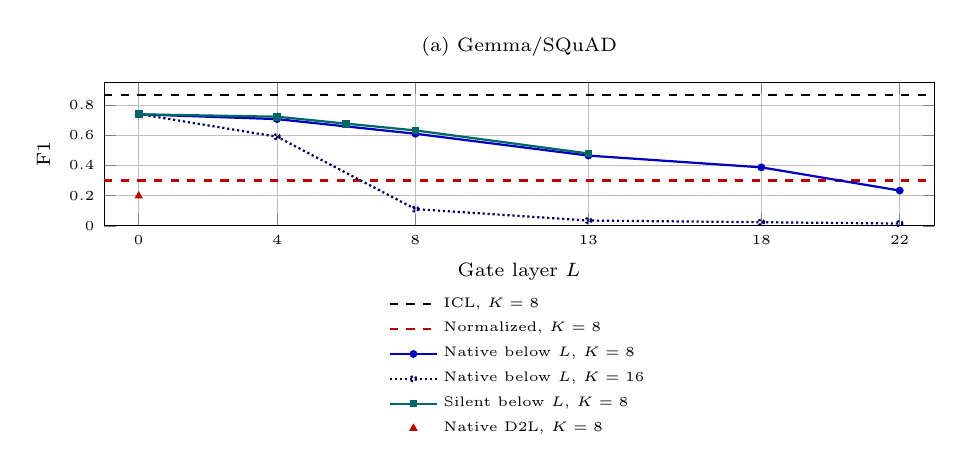
\begin{tikzpicture}
\begin{axis}[
 width=\linewidth,height=3.4cm,grid=major,
 tick label style={font=\tiny},label style={font=\scriptsize},
 title={(a) Gemma/SQuAD},title style={font=\scriptsize},
 mark size=1pt,
 xlabel={Gate layer $L$},
 ylabel={F1},xmin=-1,xmax=23,ymin=0,ymax=0.95,xtick={0,4,8,13,18,22},
  legend style={font=\tiny,draw=none,at={(0.5,-0.42)},anchor=north,
  legend columns=1,cells={anchor=west}}]
\addplot[black,dashed,thick] coordinates {(-1,.870)(23,.870)};
\addlegendentry{ICL, $K=8$}
\addplot[red!75!black,dashed,thick] coordinates {(-1,.301)(23,.301)};
\addlegendentry{Normalized, $K=8$}
\addplot[blue!75!black,mark=*,thick] coordinates {(0,.740)(4,.708)(8,.611)(13,.466)(18,.388)(22,.234)};
\addlegendentry{Native below $L$, $K=8$}
\addplot[blue!40!black,mark=o,thick,densely dotted] coordinates {(0,.742)(4,.591)(8,.111)(13,.035)(18,.024)(22,.015)};
\addlegendentry{Native below $L$, $K=16$}
\addplot[teal!80!black,mark=square*,thick] coordinates {(0,.740)(4,.724)(6,.678)(8,.633)(13,.480)};
\addlegendentry{Silent below $L$, $K=8$}
\addplot[red!75!black,mark=triangle*,thick,only marks] coordinates {(0,.198)};
\addlegendentry{Native D2L, $K=8$}
\end{axis}
\end{tikzpicture}
\end{minipage}\hfill
\begin{minipage}[t]{.49\columnwidth}
\vspace{0pt}
\centering
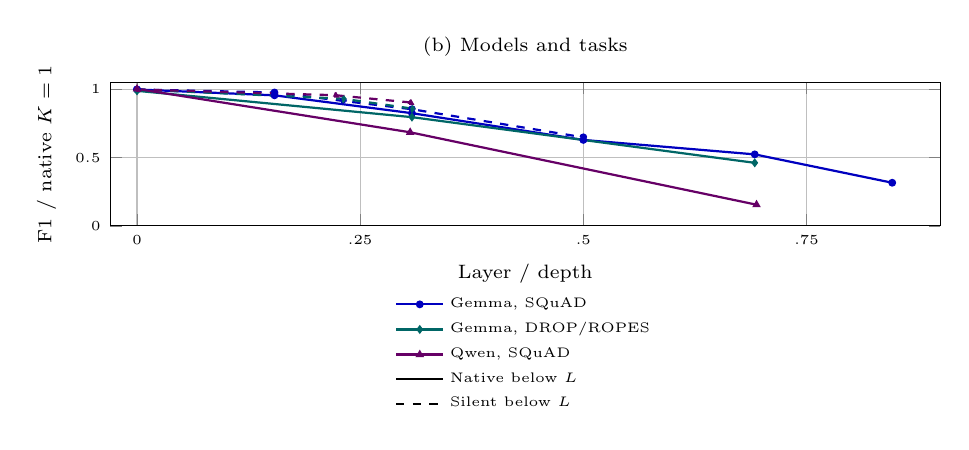
\begin{tikzpicture}
\begin{axis}[width=\linewidth,height=3.4cm,grid=major,
 tick label style={font=\tiny},label style={font=\scriptsize},
 title={(b) Models and tasks},title style={font=\scriptsize},
 xlabel={Layer / depth},ylabel={F1 / native $K=1$},
 xmin=-0.03,xmax=0.9,ymin=0,ymax=1.05,
 xtick={0,.25,.5,.75},xticklabels={0,.25,.5,.75},
 legend style={font=\tiny,draw=none,at={(0.5,-0.42)},anchor=north,
 legend columns=1,cells={anchor=west}},
 mark size=1pt]
\addplot[blue!75!black,mark=*,thick] coordinates {(0,1)(0.154,.957)(0.308,.826)(0.5,.630)(0.692,.524)(0.846,.316)};
\addlegendentry{Gemma, SQuAD}
\addplot[blue!75!black,mark=*,thick,dashed,forget plot] coordinates {(0,1)(0.154,.978)(0.231,.916)(0.308,.855)(0.5,.649)};
\addplot[teal!80!black,mark=diamond*,thick] coordinates {(0,.990)(0.308,.797)(0.692,.462)};
\addlegendentry{Gemma, DROP/ROPES}
\addplot[teal!80!black,mark=diamond*,thick,dashed,forget plot] coordinates {(0,1)(0.231,.932)(0.308,.860)};
\addplot[violet!80!black,mark=triangle*,thick] coordinates {(0,1.004)(0.306,.686)(0.694,.155)};
\addlegendentry{Qwen, SQuAD}
\addplot[violet!80!black,mark=triangle*,thick,dashed,forget plot] coordinates {(0,1)(0.222,.958)(0.306,.905)};
\addlegendimage{black,thick}
\addlegendentry{Native below $L$}
\addlegendimage{black,thick,dashed}
\addlegendentry{Silent below $L$}
\end{axis}
\end{tikzpicture}
\end{minipage}
\caption{Layer sensitivity to distractors. (a) Absolute F1 on Gemma/SQuAD.
(b) Across models and tasks at $K=8$, normalized by model depth and native
$K=1$ accuracy. Distractors are removed from layer $L$ onward.}
\label{fig:layers}
\label{fig:layer-generality}
\end{figure}

\begin{figure}[t]
\centering
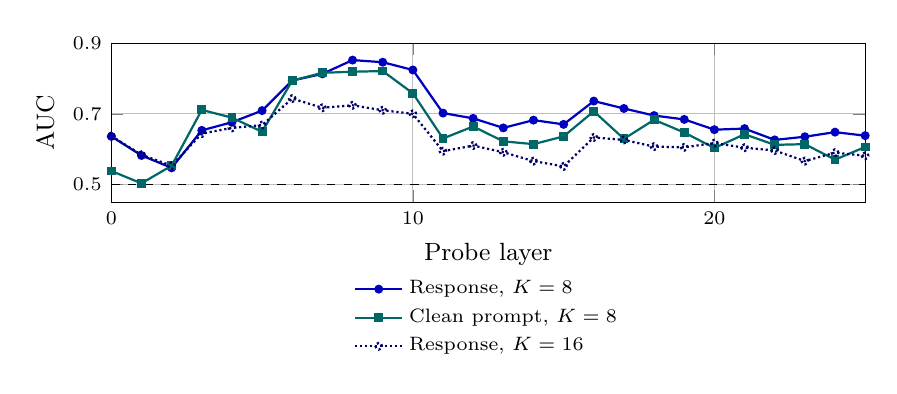
\begin{tikzpicture}
\begin{axis}[width=.92\columnwidth,height=3.6cm,grid=major,
 tick label style={font=\scriptsize},label style={font=\small},
 xlabel={Probe layer},ylabel={AUC},
 xmin=0,xmax=25,ymin=.45,ymax=.9,
 xtick={0,10,20},ytick={.5,.7,.9},
 legend style={font=\scriptsize,draw=none,at={(0.5,-0.42)},anchor=north,
 legend columns=1,cells={anchor=west}}]
\addplot[black,dashed,thin,forget plot] coordinates {(0,.5)(25,.5)};
\addplot[blue!75!black,mark=*,mark size=1.2pt,thick] coordinates {
(0,.636)(1,.582)(2,.547)(3,.653)(4,.676)(5,.709)(6,.794)(7,.813)(8,.852)(9,.846)(10,.824)
(11,.702)(12,.687)(13,.660)(14,.682)(15,.670)(16,.736)(17,.715)(18,.695)(19,.684)(20,.655)
(21,.658)(22,.626)(23,.635)(24,.648)(25,.638)};
\addlegendentry{Response, $K=8$}
\addplot[teal!80!black,mark=square*,mark size=1.2pt,thick] coordinates {
(0,.538)(1,.503)(2,.553)(3,.711)(4,.689)(5,.649)(6,.794)(7,.816)(8,.819)(9,.821)(10,.758)
(11,.630)(12,.664)(13,.622)(14,.614)(15,.636)(16,.707)(17,.629)(18,.683)(19,.647)(20,.603)
(21,.642)(22,.612)(23,.614)(24,.570)(25,.606)};
\addlegendentry{Clean prompt, $K=8$}
\addplot[blue!40!black,mark=o,mark size=1.2pt,thick,densely dotted] coordinates {
(0,.637)(1,.584)(2,.553)(3,.644)(4,.660)(5,.668)(6,.743)(7,.717)(8,.724)(9,.710)(10,.700)
(11,.594)(12,.610)(13,.591)(14,.566)(15,.551)(16,.633)(17,.626)(18,.607)(19,.605)(20,.617)
(21,.604)(22,.596)(23,.566)(24,.590)(25,.581)};
\addlegendentry{Response, $K=16$}
\end{axis}
\end{tikzpicture}
\caption{Source-membership predictability by layer. Probe AUC on Gemma;
the dashed line marks chance.}
\label{fig:layer-probes}
\end{figure}
